\documentclass[11pt, oneside]{article}   	% use "amsart" instead of "article" for AMSLaTeX format
\usepackage{geometry}                		% See geometry.pdf to learn the layout options. There are lots.
\geometry{letterpaper}                   		% ... or a4paper or a5paper or ... 
%\geometry{landscape}                		% Activate for for rotated page geometry
%\usepackage[parfill]{parskip}    		% Activate to begin paragraphs with an empty line rather than an indent
\usepackage{graphicx}				% Use pdf, png, jpg, or eps� with pdflatex; use eps in DVI mode
								% TeX will automatically convert eps --> pdf in pdflatex		
\usepackage{amssymb}
\usepackage{amsmath}
\usepackage{parskip}
\usepackage{color}
\usepackage{hyperref}

\title{Electric dipole}
%\author{The Author}
%\section{}
%\subsection*{}
\date{}							% Activate to display a given date or no date

\graphicspath{{/Users/telliott_admin/Dropbox/Tex/png/}}
% \begin{center} 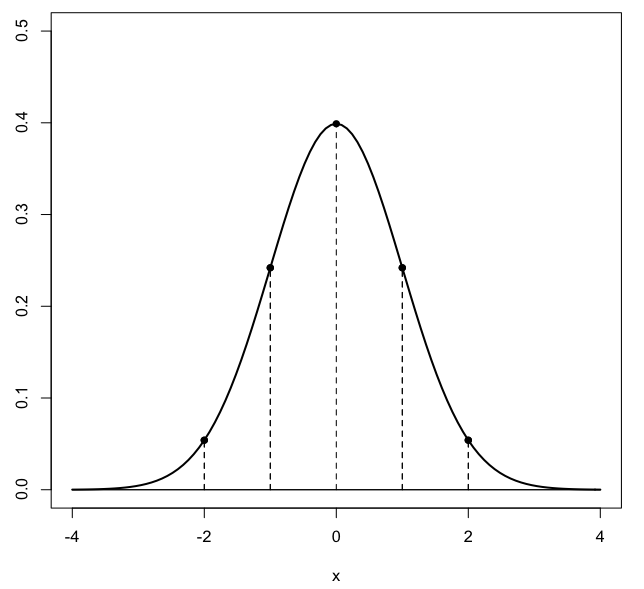
\includegraphics [scale=0.4] {gauss3.png} \end{center}
\begin{document}
\maketitle
\Large
Suppose we consider an electric dipole with two charges $+q$ and $-q$, each a distance $a$ from the origin along the $x$-axis (so their separation is $2a$).  We wish to calculate the electric field along two special lines, namely, the $x$ and $y$-axes.

For the first one, suppose the test charge lies to the right, so that it is closer to the positive charge $+q$.  The electric field is the sum of the fields for each of the two charges.  We write
\[ \mathbf{E} = \frac{q}{4 \pi \epsilon_0} \ ( \frac{1}{(r-a)^2} - \frac{1}{(r+a)^2} ) \ \hat{\mathbf{i}} \]
We can manipulate the part in the parentheses as follows:
\[ \frac{1}{(r-a)^2} - \frac{1}{(r+a)^2} = \frac{(r + a)^2 - (r - a)^2}{(r+a)^2 (r-a)^2}\]
\[ = \frac{(r^2 + 2ar + a^2) - (r^2 - 2ar + a^2)}{(r+a)^2 (r-a)^2}\]
\[ = \frac{4ar}{(r+a)^2 (r-a)^2}\]
We will combine a factor of $2a$ with $q$ as the dipole moment
\[ p = 2aq \]
leaving another $2r$ to account for.  If we expand the denominator we obtain
\[ (r+a)^2 (r-a)^2 \]
\[ = (r^2 + 2ar + a^2)(r^2 - 2ar + a^2) \]
\[ = r^4 -2r^3a + r^2a^2 + 2ar^3 - 4r^2a^2 + 2ra^3 + a^2r^2 - 2ra^3 + a^4 \]
We are interested in $r \gg a$ so we will only keep terms in $a$ but not $a^2$
\[ = r^4 -2r^3a + 2ar^3 = r^4 \]
Thus
\[ \mathbf{E} = \frac{p}{2 \pi \epsilon_0 r^3} \ \hat{\mathbf{i}} \]

For the other one, along the $y$-axis, suppose the separation from the origin is again $r$.  The vertical component of the field from $+q$ (in the positive $\hat{\mathbf{j}}$ direction), is just canceled by the vertical component of the field from $-q$.  What remains are two identical components that point in the $- \hat{\mathbf{i}}$ direction with magnitude
\[ \frac{q}{4 \pi \epsilon_0} \ \frac{1}{(a^2 + r^2)} \cos \phi \]
The sum is
\[ \mathbf{E} = - \frac{q}{2 \pi \epsilon_0} \ \frac{r}{(a^2 + r^2)^{3/2}} \]

Approximation for this??


\end{document}  